\chapter{Teil A}
\label{cha:TeilA}
Im Folgenden Kapitel wird Teil A dieser Arbeit behandelt. Es wird die Ansteuerung von TFT Displays über den 8080-Bus auf Basis des Gnublin Linuxboards realisiert. Hierzu wurden verschieden große LCD Displays mit unterschiedlichen Controllern unter Verwendung des 8080-Interface und untersucht. 

\section{Untersuchte Displays mit 8080-Interface}
Dieser Abschnitt behandelt die untersuchten Displays. Es wurden drei Displays aus China untersucht. Der Fokus bei der Bestellung lag vor allem darauf, dass die Pinbelegung der jeweiligen Displays übereinstimmen. So ist die Entwicklung von nur einer Adapterplatine zwischen Gnublin und Display nötig. Alle verwendeten Displays werden im 16 Bit Farbmodus betrieben. Die hieraus resultierende Farbtiefe beträgt 65.535 Farben.\newline % \footnote{2^16 = 65.536}
Alle verwendeten Displays arbeiten dahingehend gleich, dass sie Kommandos und Daten auf dem Datenbus anliegen, diese jedoch durch eine gesonderte Leitung unterschieden werden. Soll dem Display also etwas mitgeteilt werden, so muss zuerst ein entsprechendes Kommando und im Anschluss die Nutzdaten gesendet werden. Um Pixeldaten an das Display zu senden, hat sich die Vorgehensweise etabliert, eine Rechteckige Region im RAM des Displays zu reservieren, das durch die 4 Eckpunkte des Rechtecks definiert sind. Werden im Anschluss Pixeldaten gesendet, inkrementiert der Controller die Adresse automatisch und springt bei einem Zeilenumbruch automatisch an die richtige Stelle im RAM. Der maximale Speicher im Controller beschränkt die maximale Auflösung der ansteuerbaren TFT-Panel. Trotz der Tatsache, dass sich die Displays auf elektrischer Seite nicht unterscheiden, so müssen diese allerdings alle speziell softwareseitig behandelt werden. \todo{bild von Ramfenster hinzufuegen}

\subsection{4.3"'/5"' mit SSD1963}
Die Wahl des Controllers SSD1963 von Solomon Systech liegt nahe, da dieser bereits mit einem 4.3"'  Panel in einer vorausgehende Arbeit verwendet wird. Dort ist das Display mittels GPIO-Pins am Raspberry Pi angeschlossen. Die Software bezüglich der reinen Displayansteuerung ist somit bereits vorhanden (siehe \cite{Schlegel2013}). Aufgrund eines Problems, das in Abschnitt \ref{cha:TeilAKnownBugs_SSD1963} näher beschrieben ist, wird für diese Arbeit zusätzlich ein anderes Display mit 5"' Panel aber selbem Controller untersucht. 
\refa{fig:8080_pinout} zeigt das Pinout der verwendeten Displays.
\begin{figure}[h]
	\centering
\fbox{	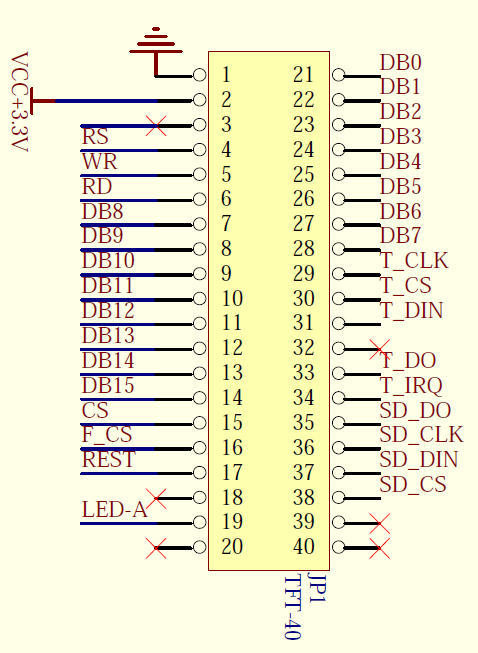
\includegraphics[width=0.5\textwidth]{TeilA/display_pinout.png}}
	\caption{8080-Display Pinout, Quelle: \cite{Coldtears2014}}
	\label{fig:8080_pinout}
\end{figure}
Die Displays besitzen bei 4.3"' eine Auflösung von 480x272 beziehungsweise bei 5"' 800x480 Pixeln. Neben den für die Initialisierung nötigen Kommandos besitzt der Controller folgende wichtigen Kommandos. Diese sind in \reft{tab:Kommandos_SSD1963} beschrieben. Die zur Initialisierung notwendigen Kommandos werden hier nicht erläutert, da diese aus dem Datenblatt entnehmbar sind.
\begin{table}[h]
\begin{tabular}{|p{4cm}|p{1cm}|p{8cm}|}\hline
\rowcolor{TableBackgroundColor} 
   \textbf{Kommando} & \textbf{Hex-Code} & \textbf{Kommentar}\\ \hline
   Set Column Address & 0x2A & Eckpunkte des RAM-Fensters in X-Richtung \\ \hline
   Set Page Address & 0x2B & Eckpunkte des RAM-Fensters in Y-Richtung \\ \hline
   Write Memory Start & 0x2C & Alle Folgenden Pixeldaten werden im RAM-Fenster platziert \\ \hline
\end{tabular}
\caption{Relevante Kommandos des SSD1963, \cite{SSD2008}}
\label{tab:Kommandos_SSD1963}
\end{table}


\subsection{3.2"' mit SSD1289}
Das 3.2"' Display von Sainsmart wird mit einen SSD1289 von Solomon Systech betrieben. Dieses Display hat eine Aufloesung ovn 320x240 Farbpunkten. Das Pinout ist dasselbe, das in \refa{fig:8080_pinout}MPMCStatic zu sehen ist. Analog zu \reft{tab:Kommandos_SSD1963} besitzt der SSD1289 seine eigenen wichtigen Kommandos. Diese sind in  \reft{tab:Kommandos_SSD1289} erlaeutert. Die zur Initialisierung notwendigen Kommandos werden hier nicht erläutert, da diese aus dem Datenblatt entnehmbar sind.
\begin{table}[h]
\begin{tabular}{|p{4cm}|p{1cm}|p{8cm}|}\hline
\rowcolor{TableBackgroundColor}
   \textbf{Kommando} & \textbf{Hex-Code} & \textbf{Kommentar}\\ \hline
   Horizontal RAM address position & 0x44 & Eckpunkte des RAM-Fensters in X-Richtung \\ \hline
   Vertical RAM address start position & 0x45 & Startpunkt des RAM-Fensters in Y-Richtung \\ \hline
   Horizontal RAM address stop position & 0x46 & Endpunkt des  RAM-Fensters in Y-Richtung \\ \hline
   Set GDDRAM X address counter & 0x4E & Zeiger im  RAM-Fenster in X-Richtung \\ \hline
   Set GDDRAM Y address counter & 0x4F & Zeiger im RAM-Fenster in Y-Richtung \\ \hline
   RAM Write  Register & 0x22 & Alle Folgenden Pixeldaten werden im RAM-Fenster platziert \\ \hline
\end{tabular}
\caption{Relevante Kommandos des SSD1289, \cite{SSD2007}}
\label{tab:Kommandos_SSD1289}
\end{table}


\subsection{5"' mit CPLD}
Als drittes Display mit 8080-Interface kommt eine 5"' Display mit einer Auflösung von 800x480 Bildpunkten zum Einsatz, dass keinen univerell einsetzbaren Controller für variable Displaypanels im klassischen Sinn besitzt, sondern ein CPLD \footnote{CPLD: Complex Programmable Logic Device} als Controller mit zugeschnittenen Timings für das verwendete TFT-Panel. Der Vorteil eines solchen Displays ist, dass keine Initialisierungsroutine benötigt wird, um die Timings für das Panel einzustellen. Ein Reset setzt das Display betriebsbereit. Nachteilig stellt sich der Umstand ein, dass nur TFT-Panels exakter Größe und mit exakten Timings verwendet werden können. Für diese Arbeit ist allerdings die Verwendung von anderen Panels belanglos. Auch hier ist das Pinout des Displays analog zu dem Gezeigten in \refa{fig:8080_pinout}.\newline
Wichtige Kommandos zum Betrieb des Displays sind in \reft{tab:Kommandos_MD050SD} einsehbar. Dieses Display trägt die Bezeichnung MD050SD.

\begin{table}[h]
\begin{tabular}{|p{4cm}|p{1cm}|p{8cm}|}\hline
\rowcolor{TableBackgroundColor}
   \textbf{Kommando} & \textbf{Hex-Code} & \textbf{Kommentar}\\ \hline
   Beginning Row Address & 0x02 & Startpunkt des RAM-Fensters in X-Richtung \\ \hline
   Ending Row Address& 0x06 & Endpunkt des RAM-Fensters in X-Richtung \\ \hline
   Beginning Column Address & 0x03 & Startpunkt des RAM-Fensters in Y-Richtung \\ \hline
   Ending Column Address& 0x07 & Endpunkt des RAM-Fensters in Y-Richtung \\ \hline
   Writing Page Register & 0x05 & Alle Folgenden Pixeldaten werden im RAM-Fenster platziert \\ \hline
\end{tabular}
\caption{Relevante Kommandos des MD050SD, \cite{ITEAD2013}}
\label{tab:Kommandos_MD050SD}
\end{table}

% \section{8080-Interface mittels GPIO-Pins}
\label{sec:TeilA_8080GPIO}

\subsection{Konzept}
\subsection{Hardwareverbindung zwischen GPIO-Pins und Display}
\subsection{User-Space-Treiber}
\subsubsection{Low-Level-Treiber}
\paragraph{GPIO-Pin Frequenz erhoehen}
\paragraph{GPIO-Treiber}
\paragraph{Displaytreiber fuer SSD1963}
\subsection{Ansteuerung des Displays}



\section{8080-Interface mittels SRAM-Interface}
\label{sec:TeilA_8080SRAM}
Wie bereits in \refc{cha:gnublin_extended} erwaehnt, besitzt der Prozessor des Gnublin bereits ein externes 8080-Interface, auf welches zugegriffen wird. Im Folgenden wird auf das Konzept, die Idee und die Realisierung auf Hardware- und Softwareseite eingegangen.
\newpage
\subsection{Konzept}
\label{cha:teila_konzept}
Im Gnublin stellt ein NXP LPC313x die zentrale Recheneinheit dar. Dieser besitzt ein sogenanntes EBI \footnote{EBI: External Bus Interface}, worüber externe Bausteine wie Speicher, Ethernetcontroller oder ähnliche Bausteine angesprochen werden können.

\begin{figure}[htp]
%\begin{minipage}[t]{0.8\textwidth}
%\begin{figure}[h]
	\centering
\fbox{	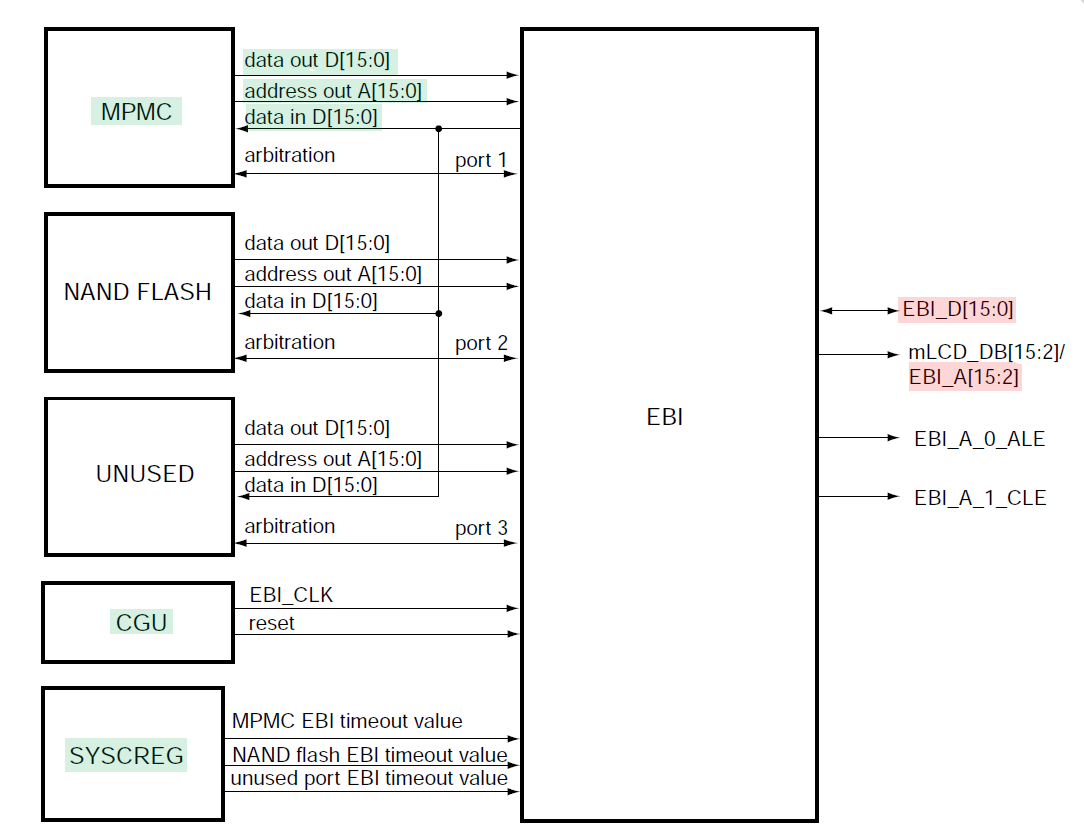
\includegraphics[width=1.0\textwidth]{TeilA/lpc_ebi.png}}
	\caption{NXP LPC313x EBI, Quelle: \cite{NXP2010}}
	\label{fig:lpc_ebi}
\end{figure}
%\end{minipage}

In \refa{fig:lpc_ebi} ist ein Blockschaltbild des EBI zu sehen, bei welchem neben CGU \footnote{CGU: Clock Generation Unit, Takterzeugung} und SYSCREG\footnote{SYSCREG: System Control Register, Steuerregister}, MPMC\footnote{MPMC: Multiport Memory Controller} sowie das NAND Flash an den Eingängen des EBI angeschlossen sind. Abgesehen von NAND Flash sind die Eingänge zum EBI für diese Arbeit relevant und grün markiert. An den Ausgängen des EBI sind Adress- und Datenbus zum Anschluss an externe Bausteine herausgeführt. Damit verschiedenartigen Bausteine an denselben Adress- und Datenpins angeschlossen werden kann, ist eine Priorisierung notwendig. Die Höchste Priorität besitzt der MPMC, gefolgt vom NAND Flash. 
Die Grundidee ist, das Display über den MPMC anzuschließen, da er so konfiguriert werden kann, dass er sich 8080-konform verhält. Die für diese Arbeit interessanten Leitungen am Ausgang des EBI sind mit rot markiert. Hier wird der Datenbus selbst, sowie die oberen 13 Bit des Adressbus gezeigt.


\subsection{MPMC - Multiport Memory Controller des NXP LPC313x}
\label{cha:mpmc}

Der MPMC stellt die Möglichkeit zur Verfügung Bausteine wie dynamisches und statisches RAM anzubinden. Die Refresh-Zyklen werden bei Verwendung von dynamischen RAMs automatisch vollzogen. Das SDRAM-Interface bietet von Haus aus die Möglichkeit Displays mit 8080-Interface zu betreiben. Dies schließt allerdings die Verwendung von dynamischen RAMs aus. Soll ein Betriebssystem wie Linux auf dem System betrieben werden, ist allerdings die Verwendung von dynamischem RAM unerlässlich. Im Folgenden wird die Schnittstelle für das statische RAM SRAM-Interface benannt. Es besteht die Möglichkeit das Interface des statischen RAM zu verwenden, um ein Display zu betreiben, da es sich so konfigurieren lässt, dass es sich wie ein 8080-Interface verhält. Damit sich die verschiedenen Slaves an Adress- und Datenbus nicht überschneiden, regelt das EBI den Zugriff auf die Busse über Chip-Select Leitungen. Am Gnublin ist eine dieser Chip-Select-Leitungen für das SRAM-Interface nach außen gelegt. Die restlichen Anschlüsse wie Write-Enable, Read-Enable, Reset sind ebenfalls herausgeführt \cite{NXP2010}. Ein Blockschaltbild des MPMC ist in \refa{fig:lpc_mpmc} zu sehen.


\begin{figure}[tbph]
%\begin{figure}[h!]
	\centering
\fbox{	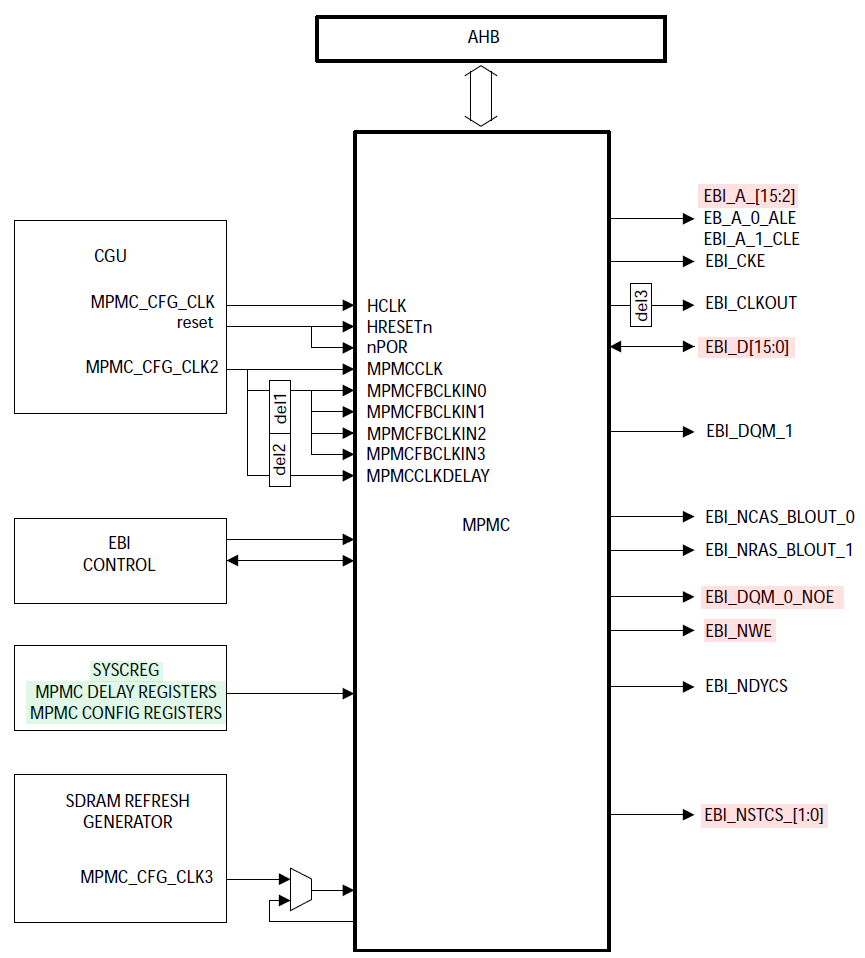
\includegraphics[width=1.0\textwidth]{TeilA/lpc_mpmc.png}}
	\caption{NXP LPC313x MPMC, \cite{NXP2010} }
	\label{fig:lpc_mpmc}
\end{figure}
\newpage
Die Register des MPMC werden so konfiguriert, dass die Schnittstelle kompatibel zum Display und dessen Timings wird. Entsprechend dem verwendeten Chip-Select-Signal werden die Register \begin{itemize}
\item MPMCStaticConfig0\item  MPMCStaticWaitWen0\item  MPMCStaticWaitOen0\item  MPMCStaticRd0\item  MPMCStaticPage0\item  MPMCStaticWr0 \item MPMCStaticWaitTurn0 \end{itemize} konfiguriert. Die Basisadresse des MPMC ist 0x1700 8000. Wie die Register zu beschreiben sind, geht aus \cite{NXP2010} auf Seite 56 hervor und ist in \reft{tab:mpmc_config} gezeigt. Die Timings wurden so gewählt, dass die Timinganforderungen der Displaycontroller eingehalten werden.

\begin{table}[h]
\begin{tabular}{|p{4cm}|p{1cm}|p{1cm}|p{6.6cm}|}\hline
\rowcolor{TableBackgroundColor} 
	\textbf{Register} 	& \textbf{Offset} 	& \textbf{Wert} & \textbf{Beschreibung} 							\\ \hline
	MPMCStaticConfig0 	& 0x200 		& 0x81 			& \begin{itemize}
	\item 16 Bit Modus \item Aktiviert die Nutzung von EBI\_nWE \item  CS low aktiv\item  keine ExtendedWait-Zyklen\item  Schreibpuffer deaktiviert\item  Geschütztes Schreiben deaktiviert \item Page Mode deaktiviert 	\end{itemize} 	\\ \hline
	MPMCStaticWaitWen0 	& 0x204 		& 13 			& 13 + 1 = 14 Wartezyklen ab Chip-Select bis Write-Enable 	\\ \hline
	MPMCStaticWaitOen0 	& 0x208 		& 0 			& 0 + 1 = 1 Wartezyklus ab Chip-Select bis Output-Enable  												\\ \hline
	MPMCStaticRd0 		& 0x20C 		& 0 			& 0 + 1 = 1 Wartezyklus ab Chip-Select bis Read-Enable					\\ \hline
	MPMCStaticPage0 	& 0x210 		& 0 			& 0 + 1 = 1 Wartezyklus für sequential Page Mode Access												\\ \hline
	MPMCStaticWr0 		& 0x214 		& 15 			& 15 + 2  = 17 Wartezyklen bis Write-Access	\\ \hline
	MPMCStaticWaitTurn0 & 0x218 		& 0 			& 0 + 1 = 1 Turnaround Cycles 								\\ \hline
\end{tabular}
\caption{MPMC Register, \cite{NXP2010}}
\label{tab:mpmc_config}
\end{table}
\newpage

Neben den MPMC-Registern muss das Register SYSCREG\_AHB\_MPMC\_MISC konfiguriert werden. Wird Bit 7 des Registers  auf der Adresse 0x1300 2864 mit dem Wert 0 eingestellt, so verändert sich das Adressierungsverhalten dahingehend, dass sich die Adressleitungen des EBI EBI\_A[15:0] auf den für den Prozessor sichtbaren AHB\footnote{AHB: Advanced Microcontroller Bus Architecture} Adressbus AHB\_A[16:1] verschiebt (siehe \cite{NXP2010}, S.~485f). Der Prozessor selbst, kann nun also 17 Bit adressieren, jedoch nur im Sprung von zwei Adressen, da das ursprüngliche LSB weggefallen ist.

\newpage
\subsection{Hardwareverbindung zwischen SRAM-Interface und Display}
In diesem Abschnitt wird die Verbindung zwischen dem Prozessor und dem Display behandelt. Eingangs wurde bereits erwähnt, dass beim Kauf der Displays Augenmerk auf Pinkompatibilität gelegt wurde. Das schlägt sich beim Entwurf der Adapterplatine positiv zu Buche, da nun lediglich ein Adapter benötigt wird. \newline
Bereits dargestellt zeigt \refa{fig:8080_pinout} auf Seite \pageref{fig:8080_pinout} das Pinout der verwendeten Displays. Der Anschluss an den Prozessor stellt sich wir in \reft{tab:display_gnublin_verbindung} dar. Anhand der gewonnenen Erkenntnisse aus \refc{cha:teila_konzept} und \refc{cha:mpmc} sowie des Schaltplans des verwendeten Gnublin Extended (siehe \cite{EmbeddedProjects2013}) kann eine Zuordnung getroffen werden. Nicht verbundene Pins sind mit 'nc'\footnote{nc: not connected} vermerkt.

\begin{table}[h]
\begin{tabular}{|p{0.6cm}|p{2.5cm}|p{2.5cm}|p{0.6cm}|p{2.5cm}|p{2.5cm}|}\hline
\rowcolor{TableBackgroundColor} 
\textbf{Nr.}	&	\textbf{Pin Display}	&	\textbf{Pin Gnublin}  & \textbf{Nr.}	&	\textbf{Pin Display}	&	\textbf{Pin Gnublin} 	\\ \hline
1				&	GND						&	GND					  &	21				&	DB0						&	LPC\_DB0				\\ \hline
2				&	+3V3					&	+3V3				  &	22				&	DB1						&	LPC\_DB1				\\ \hline
3				&	nc						&	nc				 	  & 23				&	DB2						&	LPC\_DB2				\\ \hline
4				&	RS						&	LPC\_A15	    	  &	24				&	DB3						&	LPC\_DB3				\\ \hline
5				&	WR						&	LPC\_WE				  &	25				&	DB4						&	LPC\_DB4				\\ \hline
6				&	RD						&	LPC\_DQM0			  &	26				&	DB5						&	LPC\_DB5				\\ \hline
7				&	DB8						&	LPC\_DB8			  &	27				&	DB6						&	LPC\_DB6				\\ \hline
8				&	DB9						&	LPC\_DB9			  &	28				&	DB7						&	LPC\_DB7				\\ \hline
9				&	DB10					&	LPC\_DB10			  &	29				&	nc						&	nc						\\ \hline
10				&	DB11					&	LPC\_DB11			  &	30				&	nc						&	nc						\\ \hline
11				&	DB12					&	LPC\_DB12			  &	31				&	nc						&	nc						\\ \hline
12				&	DB13					&	LPC\_DB13			  &	32				&	nc						&	nc						\\ \hline
13				&	DB14					&	LPC\_DB14			  &	33				&	nc						&	nc						\\ \hline
14				&	DB15					&	LPC\_DB15			  &	34				&	nc						&	nc						\\ \hline
15				&	CS						&	STCS0				  &	35				&	nc						&	nc						\\ \hline
16				&	nc						&	nc					  &	36				&	nc						&	nc						\\ \hline
17				&	RESET					&	GPIO19				  &	37				&	nc						&	nc						\\ \hline
18				&	nc						&	nc					  &	38				&	nc						&	nc						\\ \hline
19				&	LED-A					&	GPIO20				  &	39				&	nc						&	nc						\\ \hline
20				&	nc						&	nc				 	  &	40				&	nc						&	nc						\\ \hline

\end{tabular}
\caption{Displayverbindung mit dem Gnublin, \cite{Coldtears2014}, \cite{EmbeddedProjects2013}}
\label{tab:display_gnublin_verbindung}
\end{table}

Das Daten-Interface des Displays ist mit den Pins DB[0:15] mit dem Datenbus verbunden. Die Signale Read-Enable RD und Write-Enable WR liegen auf den Pins LPC\_DQM0 und LPC\_WE. Als Chip-Select wird das Signal STCS0 verwendet. Diese Pins sind aus dem EBI herausgeführt (siehe \refa{fig:lpc_ebi}) und werden, sofern es das System von der Auslastung am Bus ermöglicht, für das Display zur Verfügung gestellt.

Das RS Signal am Display, welches zwischen Kommando und Daten unterscheidet, liegt auf dem Adresssignal A15. Die folgenden Angaben gehen von einer Registerkonfiguration nach \refc{cha:mpmc} aus. Werden Daten gesendet, so ist der Pin logisch 1, was einem Wert auf dem Adressbus von 0x10000\footnote{0x10000 = 0b0001 0000 0000 0000 0000} entspricht. Bei Kommandos ist der Pin logisch 0 mit einem Adresswert von 0x00000\footnote{0x00000 = 0b0000 0000 0000 0000 0000}. Die unteren 16 Bits des Adressraums lassen sich also willkürlich verändern, da nur das MSB\footnote{MSB: Most Sigificant Bit, das höchstwertige Bit} vom Display verwendet wird. 

Als RS-Pin ist die Adressleitung A15 (logisch verschoben auf A16) gewählt, da so möglicherweise DMA-Transfers\footnote{DMA: Direct Memory Access, Speichertransfer effizient und schnell direkt in Hardware} von bis zu 65.536 Bytes\footnote{65.536 = $2^{16}$} möglich sind. Der DMA-Transfer könnte die Adressleitungen bei Daten von 0x10000 bis 0x1FFFF\footnote{0x1FFFF = 0b0001 1111 1111 1111 1111} bzw. bei Kommandos von 0x0000 bis 0x0FFFF\footnote{0x0FFFF = 0b0000 1111 1111 1111 1111} inkrementieren ohne die Gültigkeit der Wahl zwischen Kommando und Daten des Displays zu beeinträchtigen.

Das Display lässt sich Zusammenfassend also über zwei Pseudoregister für Kommando und Daten auf den Adressoffsets 0x00000 und 0x10000 mit der Basisadresse 0x20000000 ansprechen. Dies ist in \reft{tab:sram_adressen} nochmals übersichtlich dargestellt.

\begin{table}[h]
\begin{tabular}{|p{4.5cm}|p{4cm}|p{4cm}|}\hline
\rowcolor{TableBackgroundColor} 
	\textbf{Register} 	& \textbf{Adresse} 	& \textbf{Typ} 			\\ \hline
	SRAM0\_DISP\_CTRL 	& 0x20000000		& Kommandos				\\ \hline
	SRAM0\_DISP\_DATA 	& 0x20010000 		& Daten 				\\ \hline
\end{tabular}
\caption{Adressen für SRAM-Zugriff, \cite{NXP2010}}
\label{tab:sram_adressen}
\end{table}


Die Untersuchung inwieweit DMA-Transfer praktisch mit der verwendeten Hardware möglich ist, ist allerdings nicht Bestandteil dieser Arbeit. 

\newpage
\subsection{Adapterplatine zwischen Gnublin Extended und Display}
Der Adapter wird als Platine realisiert, die auf den Gnublin Extended aufgesteckt wird. Das Display wiederum wird mit der Adapterplatine steckbar verbunden. Der Schaltplan ist in \refa{fig:adapterplatine_sch} gezeigt und stellt entsprechend \reft{tab:display_gnublin_verbindung} die Verbindungen her.

Der grün markierte Bereich stellt die Verbindung zum Display dar, rot zum Gnublin Extended und im blauen Rechteck sind weitere kleine Bauteile untergebracht. Hier sind Pullup-Wiederstande mit 10~k$\Omega$ an den Leitungen STCS0, Reset und LED-A um definierte Pegel vorzugeben zu sehen sowie einen Blockkondensator mit 100~nF, der für eine bessere Spannungsversorgung des Displays sorgt.

\begin{figure}[tbph]
%\begin{figure}[h!]
	\centering
\fbox{	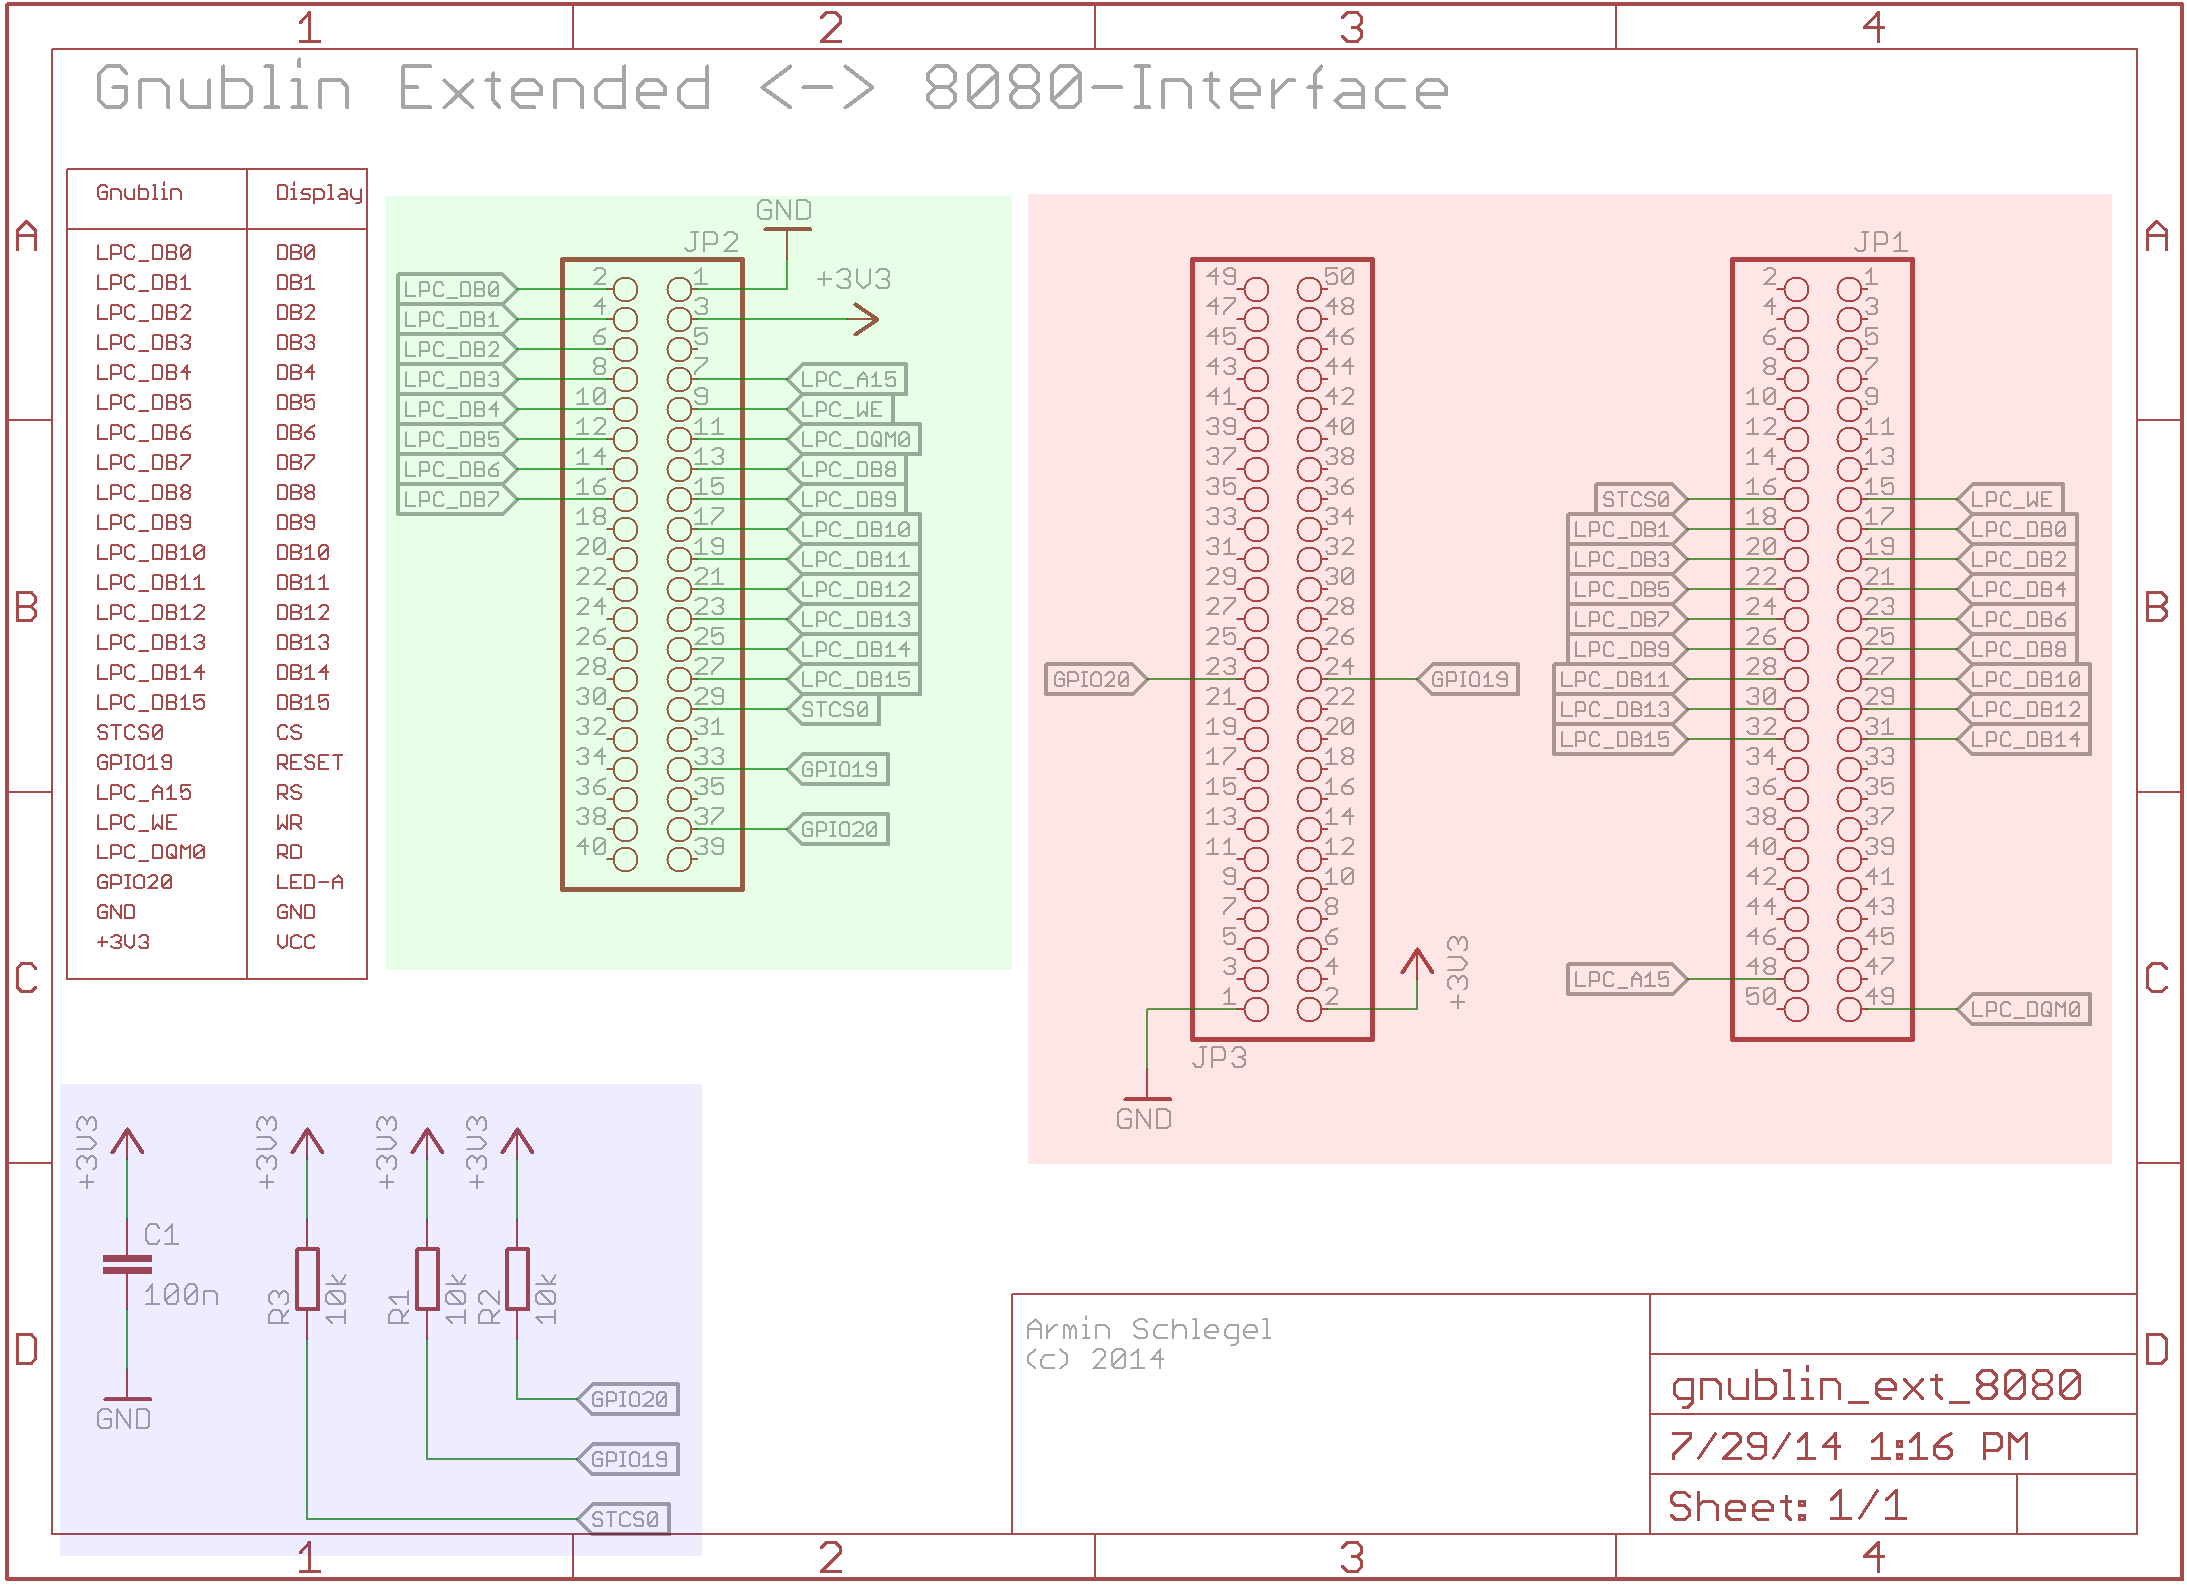
\includegraphics[width=1.0\textwidth]{TeilA/schematic.png}}
	\caption{Schaltplan Adapterplatine}
	\label{fig:adapterplatine_sch}
\end{figure}
\newpage

\refa{fig:adapterplatine} (a) und (b) zeigt je ein gerendertes 3D Bild der Ober- und Unterseite der Adapterplatine. Auf der Oberseite wird das Display auf der linken Seite mit der 40 poligen Stiftleiste angeschossen. Mit der Unterseite wird die Platine auf das Gnublin Extended mit je zwei 50 poligen Buchsenleisten aufgesteckt.

\begin{figure}
        \begin{center}
        \begin{subfigure}[htp]{0.8\textwidth}
                \fbox{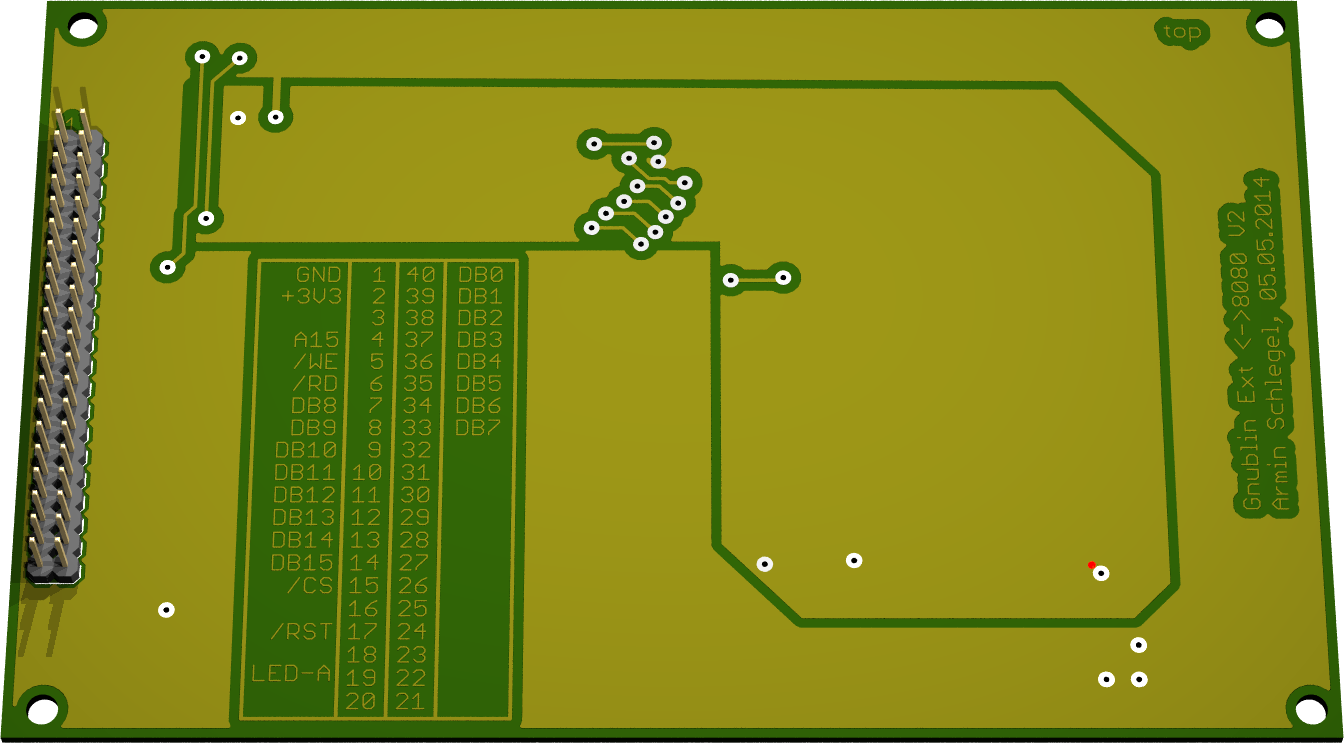
\includegraphics[width=\textwidth]{TeilA/gnublin_ext_ssd1963_top.png}}
                \caption{Adapterplatine Top Layer}
                \label{fig:adapter_top}
        \end{subfigure}

        \begin{subfigure}[htp]{0.8\textwidth}
               \fbox{ 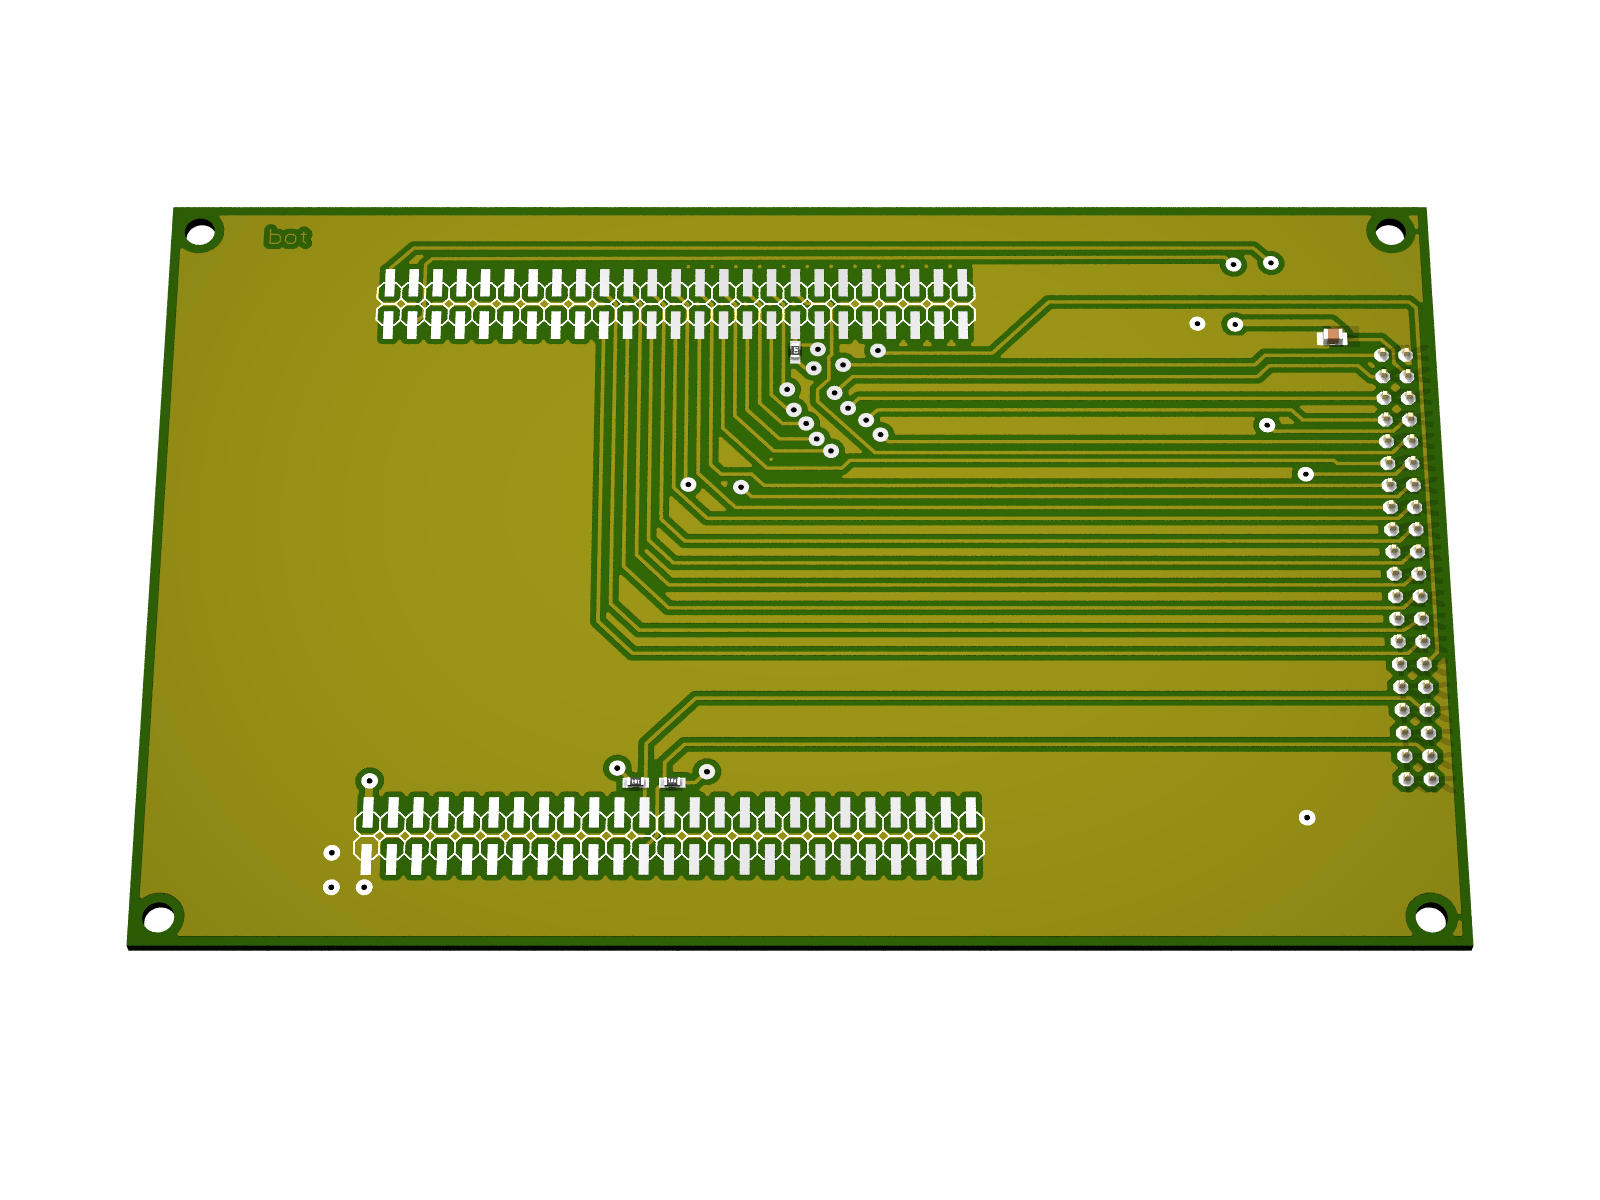
\includegraphics[width=\textwidth]{TeilA/gnublin_ext_ssd1963_bot.png} }              				\caption{Adapterplatine Bottom Layer}
                \label{fig:adapter_bot}
        \end{subfigure}
		\end{center}
        \caption{Adapterplatine zwischen Gnublin Extended und Display}\label{fig:adapterplatine}
\end{figure}

Die Schaltplan und das Layout befinden sich in der CD im Anhang dieser Arbeit.
\newpage
\subsection{Software}
Im Folgenden Abschnitt wird die Software behandelt, die nötig ist, um das Display zu betreiben. 
Die Softwareentwicklung ist in drei Teile auf gegliedert:
\begin{itemize}
\item Modifikationen im Bootloader APEX
\item Userspace-Treiber basierend auf einem Treibers auf für den Raspberry Pi (siehe \cite{Schlegel2013a} und \cite{Schlegel2013b}) bei dem mittels GPIO-Pins ein 8080-Display zu betreiben
\item Framebuffer-Treiber im Linux-Kernel
\end{itemize}

\subsubsection{Anpassung des APEX-Bootloaders zur Verwendung des Displays}
Der APEX-Bootloader\footnote{\url{https://gitorious.org/apex/}} wurde ursprünglich für Prozessoren de Sharp LH Familie entwickelt, wurde allerdings auf eine Vielzahl von weiteren ARM basierten Prozessoren portiert, so auch für die verwendete NXP LPC313x CPU\footnote{CPU: Central Processing Unit, Prozessor}.
Die Aufgabe des Bootloaders ist es, grundlegende prozessorinterne Hardwareeinheiten wie z.B. CGU oder SD-RAM zu initialisieren um für den Linux-Kernel die notwendige Umgebung zu schaffen. Im Anschluss wird der Linux-Kernel geladen und gestartet. Es werden außerdem dem Linux-Kernel Bootparameter übergeben, die zum Start benötigt werden. Am Anfang des Bootloader-Codes werden die verwendeten MPMC-Register konfiguriert. Wie in \refc{cha:mpmc} muss das SYSCREG-Register SYSCREG\_AHB\_MPMC\_MISC nicht explizit beschrieben werden, da es im Resetzustand bereits richtig konfiguriert ist. \refl{lst:apex_mpmc_config} zeigt die entsprechende Initialisierung der MPMC-Register für das MD050SD. Die Adressen von z.B. MPMC\_STCONFIG0 sind in der \lstinline|lpc313x.h| definiert. Die Modifikationen im Bootloader finden in der Datei \lstinline|initialize.c| statt.

\begin{lstlisting}[%
language=MyC,
caption={Bootloader: MPMC-Konfiguration},
label=lst:apex_mpmc_config
]
#elif defined(CONFIG_MACH_EPLPC3131_V1)
#if defined(CONFIG_DISP_SSD1963)
	// ...
#elif defined(CONFIG_DISP_MD050SD)
   /* LCD display, 16 bit */
   MPMC_STCONFIG0  = 0x81;
   MPMC_STWTWEN0   = 13;
   MPMC_STWTOEN0   = 0;
   MPMC_STWTRD0    = 0;
   MPMC_STWTPG0    = 0;
   MPMC_STWTWR0    = 15;
   MPMC_STWTTURN0  = 0;
#elif defined(CONFIG_DISP_SSD1289)
	// ...
#elif defined(CONFIG_DISP_NONE)
	// ...
#endif
#endif
\end{lstlisting}


\paragraph{Boot-Logo im APEX-Bootloader}
Um dem Display beim Systemstart einen initialisierten Zustand zu geben und dem Benutzer bereits während dem Laden des Linux-Kernels ein Bild anzuzeigen, ist ein Bootlogo konfigurierbar. Hierfür bedarf es eines rudimentären Displaytreibers im Bootloader. Im Folgenden wird die Darstellung des Boot-Logos unter Verwendung des MD050SD dargestellt. \refl{lst:apex_erster_teil} zeigt den ersten Teil des Treibers, bei dem grundlegende Datentypen sowie Sendefunktionen für Daten und Kommandos gelistet sind. 

\begin{lstlisting}[%
language=MyC,
caption={Bootloader: Grundlegende Datentypen und Funktionen},
label=lst:apex_erster_teil
]
#if defined(CONFIG_DISP_MD050SD) || defined(CONFIG_DISP_SSD1963) || defined(CONFIG_DISP_SSD1289)
#define DISP_PHYS        (EXT_SRAM0_PHYS)
#define DISP_PHYS_CTRL   (DISP_PHYS + 0)
#define DISP_PHYS_DATA   (DISP_PHYS + 0x10000)

unsigned int width;
unsigned int height;
int pixel;

struct display {
   volatile u16* ctrl;
   volatile u16* data;
};

static struct display display;

static void display_send_cmd(u16 cmd)
{
   *display.ctrl = 0x00FF & cmd;
}

static void display_send_data(u16 data)
{
   *display.data = data;
}

#endif
\end{lstlisting}

Die Struktur \lstinline|struct display| ab Zeile 10 von \refl{lst:apex_erster_teil} enthält zwei Zeiger \lstinline|u16* ctrl| und \lstinline|u16* data| auf die jeweiligen Adressen aus \reft{tab:sram_adressen} für Kommandos und Daten. In den Zeilen 17 und 22 sind die zwei Sendefunktionen \lstinline|display_send_cmd(u16 cmd)| und 
\lstinline|display_send_data(u16 cmd)| definiert. Hiermit werden die Kommandos und Daten an das Display gesendet. Wird auf eine der beiden Adressen ein Wert geschrieben, kümmert sich das MPMC und das EBI automatisch um die restlichen Signale wie WR, RD und CS. 

\begin{lstlisting}[%
language=MyC,
caption={Bootloader: Display-Initialisierung und Bootlogo},
label=lst:apex_zweiter_teil
]
#if defined(CONFIG_DISP_MD050SD) || defined(CONFIG_DISP_SSD1963) || defined(CONFIG_DISP_SSD1289)
   display.ctrl = &__REG16 (DISP_PHYS_CTRL);   
   display.data = &__REG16 (DISP_PHYS_DATA); 
#if defined(CONFIG_DISP_MD050SD)
   GPIO_OUT_LOW(IOCONF_GPIO, _BIT(14)); //GPIO20 is LED_ENABLE

   GPIO_OUT_LOW(IOCONF_GPIO, _BIT(13)); //GPIO19 is nRESET
   udelay(20000);
   GPIO_OUT_HIGH(IOCONF_GPIO, _BIT(13)); //GPIO19 is nRESET
   udelay(20000);

	/* Set Window from 0,0 to 479, 799 */
   display_send_cmd(0x0002);			
   display_send_data(0);				
   display_send_cmd(0x0003);			
   display_send_data(0);				

   display_send_cmd(0x0006);
   display_send_data(480 - 1);
   display_send_cmd(0x0007);
   display_send_data(800 - 1);

	/* Clear the display with color black */
   display_send_cmd(0x000F);

   for(pixel = 0; pixel < 800 * 480; pixel++)
   {
      display_send_data(0x0000);
   }

   GPIO_OUT_HIGH(IOCONF_GPIO, _BIT(14)); //GPIO20 is LED_ENABLE

#if defined(CONFIG_LOGO_TUX)
   width = boot_logo_tux[0];
   height = boot_logo_tux[1];

   display_send_cmd(0x0002);
   display_send_data(480/2 - (height - 1)/2);
   display_send_cmd(0x0003);
   display_send_data(800/2 - (width - 1)/2);
   display_send_cmd(0x0006);
   display_send_data(480/2 + (height - 1)/2 + 1);
   display_send_cmd(0x0007);
   display_send_data(800/2 + (width - 1)/2 + 1);
   display_send_cmd(0x000F);

   for(pixel = 2; pixel < width * height + 2; pixel++)
   {
      display_send_data(boot_logo_tux[pixel]);
   }
#endif
#endif
#endif
\end{lstlisting}

Der Eigentliche Treiber und der Code für das Anzeigen des Bootlogos ist in \refl{lst:apex_zweiter_teil} zu sehen. In Zeile 2 und 3 werden den Adresszeigern die pysikalischen Adressen zum Schreiben von Kommandos und Daten zugewiesen. Von Zeile 5 bis 10 wird die Hintergrundbeleuchtung explizit abgschaltet und ein Reset auf das Display gegeben. Da das MD050SD einen CPLD-Controller besitzt, welcher eine auf genau dieses TFT-Panel zugeschnittene Programmierung enthält, fällt eine Initialisierungsroutine weg. Dies wäre bei Controllern wie dem SSD1963 nicht der Fall, da diese mit einer Vielzahl von Panels arbeiten können und demzufolge eine spezielle Initialisierung brauchen. Das MD050SD ist nach dem Reset also initialisiert und erwartet Kommandos. Von Zeile 13 bis 24 in \refl{lst:apex_zweiter_teil} wird ein Bereich im Display-RAM der vollen Bildschirmgröße reserviert und die Bereitschaft zum Datenempfang gestartet (siehe \reft{tab:Kommandos_MD050SD}). Alle Daten die im Anschluss gesendet werden, werden automatisch an die richtige Stelle im Display geschrieben. In einer Schleife werden ab Zeile 26 alle reservierten Pixel von zuvor mit der Farbe Schwarz beschrieben, um das automatisch angezeigte Testbild des Displays beim Start zu überschreiben. Im Anschluss wird die Hintergrundbeleuchtung wieder eingeschaltet. Ist über den Codeswitch \lstinline|CONFIG_LOGO_TUX| das Bootlogo aktiviert, so wird dies ab Zeile 34 angezeigt. Die Größe des Logos wird in den Zeilen 34 und 35 ausgelesen und in den Folgenden angezeigt. Die Pixeldaten des Logos sind im Array \lstinline|u16 boot_logo_tux[]| in den Dateien \lstinline|boot_logo_tux.c| und \lstinline|boot_logo_tux.h| hinterlegt.


\paragraph{Konfiguration des APEX-Bootloaders}
Der APEX-Bootloader besitzt zur Konfiguration dasselbe System wie der Linux-Kernel. Dieses System heißt KConfig und wird durch den Befehl \lstinline|make menuconfig| aufgerufen, welches ein Konfigurationsmenü im aufrufenden Terminal erscheinen lässt. Hier sind neben Grundlegenden Konfiguration zum Beispiel für die Prozessorarchitektur oder Taktraten auch der Displaytreiber und das Bootlogo eingepflegt. \refa{fig:apex_config} zeigt exemplarisch den Unterpunkt \lstinline|Platform Setup| bei dem das Display MD050SD und das Bootlogo ausgewählt sind. 

\begin{figure}[tbph]
%\begin{figure}[h!]
	\centering
\fbox{	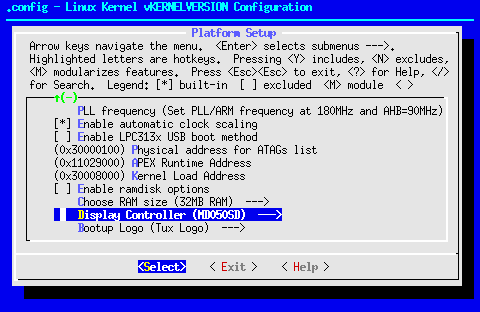
\includegraphics[width=0.8\textwidth]{TeilA/apex_config.png}}
	\caption{APEX-Bootloader KConfig}
	\label{fig:apex_config}
\end{figure}
\newpage

Bevor der Bootloader konfiguriert werden kann, muss der Vanilla-Quellcode noch gepatcht werden. \refl{lst:apex_patchen} zeigt die einzelnen Schritte, um den Bootloader herunterzuladen und zu Patchen. Der Patch enthält alle nötigen Dinge zum Betrieb des MD050SD-Display und des Boot-Logos.


\begin{lstlisting}[%
language=bash,
caption={Bootloader: Herunterladen und Patchen},
label=lst:apex_patchen
]
$ wget https://github.com/embeddedprojects/gnublin-distribution/raw/master/lpc3131/bootloader/apex/1.6.8/apex-1.6.8.tar.gz
$ tar xvfz apex-1.6.8.tar.gz
$ wget https://github.com/siredmar/master/raw/master/Teil_A/software/bootloader/apex_display.patch
$ cd apex-1.6.8
$ patch -p1 < ../apex_display.patch
\end{lstlisting}

Im Folgenden wird die Konfiguration des Bootloaders und die damit möglichen Einstellungsmöglichkeiten beschrieben. Im Konfigurationsmenü sind nach dem patchen im Untermenü \lstinline|Platform Setup| die Optionen \lstinline|Display Controller| und \lstinline|Bootup Logo| verfügbar. Hier wird die Auswahl bezüglich Displaycontrollers und Logo getroffen. Wird ein Displaycontroller anders als MD050SD gewählt, so werden nur entsprechende Timings der MPMC-Register gesetzt und kein Boot-Logo angezeigt. 
Um den Kernel mit spezifischen Parametern starten zu können, werden für den Betrieb der unterschiedlichen Treiber (Framebuffer, User-Space) andere Bootparameter benötigt. So ist der originalen Parameterliste 
\lstinline{console=ttyS0,115200n8 root=/dev/mmcblk0p3 rw rootfstype=ext4 rootwait} im Untermenü \lstinline|Environment| für den Betrieb mit dem Framebuffer-Treiber ein \lstinline|fbcon=rotate:0 fbcon=font:VGA8x16| hinzuzufügen um dem Kernel beim Start Informationen über den Kernel-Treiber \lstinline|fbcon| mitzuteilen. Wird der User-Space-Treiber verwendet, so übernimmt das Kernel-Modul \lstinline|vfb|\footnote{vfb: Virtual Frame Buffer} die Aufgabe des Framebuffers. Die Parameterliste ist mit \lstinline|console=tty0 video=vfb: vfb_enable=1| zu ergänzen (siehe \cite{LinuxKernelFBCON}).

Der Bootloader wird per \lstinline|make apex.bin| kompiliert und mit \lstinline|dd if=src/arch-arm/rom/apex.bin of=/dev/sdXY| \footnote{/dev/sdXY: bezieht sich auf die Bootpartition auf der korrekten SD-Karte, z.b. /dev/sdb2} auf die SD-Karte des Gnublin geschrieben (siehe \cite{GnublinWiki2013}).

\subsubsection{Entwicklung eines Linux-Framebuffer-Treibers}
\todo{Kernel patchen}
In diesem Abschnitt wird die Entwicklung des Framebuffer-Treibers beschrieben. Der Framebuffer-System bietet eine Abstraktionsebene für die Grafikhardware. Es enthält einen Bildspeicher der Grafikhardware und bietet Applikationen Zugriff auf diesen, ohne jedoch Informationen über die letztendlich verwendete Hardware selbst auf Low-Level-Ebene haben zu müssen. Ein Framebuffer-Device erzeugt die Node \lstinline|/dev/fbX| mit der fortlaufenden Nummer X, beginnend bei Null, für jede Instanz eines Framebuffers. Jede grafische Anwendung in einem Linux-System benötigt eine Funktionalität, die den aktuellen Bildschirminhalt speichert und  Applikationen zugriff darauf gewährt. Dabei ist es im wesentlichen unwichtig, ob die Anzeige selbst durch Hardware beschleunigt oder sogar nur rein virtuell realisiert wird, da die Applikation auf die Schnittstelle in \lstinline|/dev/fbX| zugreift (siehe  \cite{LinuxKernelFB}).
Programme wie zum Beispiel der X11-Server, Video-Player, QT\footnote{QT: C++-Klassenbibliothek zur 2D-Darstellung}, SDL\footnote{SDL: Simple Direct Media Layer, Grafikbibliothek zur 2D-Darstellung} usw. können dieses System nutzen. Gerade für leistungsschwächere Systeme bietet es dahingehend dieselben Möglichkeiten Programme Anzuzeigen, wie für High-End-Systeme. Einzig die Art und Weise des Befüllens und Auslesens des Framebuffers unterscheidet die Leistungsfähigkeit einzelner Systeme. So können Systeme mit zusätzlichen Grafikeinheiten die speziell zum Berechnen von 3D-Daten mit zum Beispiel der 3D-Grafikbibliothek OpenGL\footnote{OpenGL: 3D Grafikbibliothek} den Framebuffer mit "'hochwertigeren"' Inhalten füllen, als ein System, das diese Möglichkeit nicht besitzt. Die Abstraktionsebene für die Applikation bleiben aber dieselben. 

Mit der Entwicklung eines Framebuffer-Treibers, sind alle Vorteile erschlossen, welche das Framebuffer-System bietet. Diese sind eine standardisierte Schnittstelle für Applikationen, sowie die Gewissheit, dass, sofern es die Rechenleistung zulässt, prinzipiell alle bereits existenten Programme und Inhalte angezeigt werden können.
In den folgenden Abschnitten, wird die Entwicklung des Framebuffer-Treibers für die drei verwendeten Displays dargelegt, mit Fokus auf das MD050SD. 
\paragraph{Framebuffer-Treiber für MD050SD}
In diesem Abschnitt wird die Funktionsweise des Framebuffer-Treibers für das MD050SD beschrieben. Auf ein Listing des kompletten Treibers wird an dieser Stelle bewusst verzichtet, sondern nur die elementaren Funktionen und Gedanken aufgezeigt.

Der Treiber arbeitet konform mit dem "'Platform Device"'- und "'Platform Driver"'-System im Linux-Kernel (siehe \cite{LinuxKernelPlatformDeviceDriver}). Mit dem Platform-Device-System wird ein Pseudo-Bus erzeugt, mit dem sich verschiedene Platform-Driver verbinden können. So können beispielsweise mehrere voneinander unabhängige Instanzen eines Treibers oder vieler verschiedener Treiber im System verfügbar sein. Beinhaltet ein System ein Platform-Device, so muss es dem Linux-Kernel bekannt gemacht werden. Hierzu wird die Struktur \lstinline|struct platform_device| verwendet, die in \refl{lst:struct_platform_device} gezeigt ist.

\begin{lstlisting}[%
language=MyC,
caption={Framebuffer: struct platform\_device},
label=lst:struct_platform_device
]
struct platform_device {
	const char	*name;
	u32		id;
	struct device	dev;
	u32		num_resources;
	struct resource	*resource;
};
\end{lstlisting}

In der Struktur in \refl{lst:struct_platform_device} sind Datentypen enthalten, die einen eindeutigen Namen des Devices \lstinline|const char *name|, sowie eine ID \lstinline|u32 id|  bestimmen, einen Parameter zur Struktur \lstinline|struct device|, sowie einen Zeiger zur Struktur \lstinline|strut resource|, die letztendlich die Hardware-Ressourcen darstellen. Für den Platform-Driver ist die Struktur \lstinline|struct platform_driver| in \refl{lst:struct_platform_driver} gegeben, die Funktionszeiger für den Betrieb des Treibers und eine Struktur \lstinline|struct device_driver| enthält, welche zur Zuordnung mit dem entsprechenden Platform-Device dient.
\begin{lstlisting}[%
language=MyC,
caption={Framebuffer: struct platform\_driver},
label=lst:struct_platform_driver
]
struct platform_driver {
	int (*probe)(struct platform_device *);
	int (*remove)(struct platform_device *);
	void (*shutdown)(struct platform_device *);
	int (*suspend)(struct platform_device *, pm_message_t state);
	int (*suspend_late)(struct platform_device *, pm_message_t state);
	int (*resume_early)(struct platform_device *);
	int (*resume)(struct platform_device *);
	struct device_driver driver;
};
\end{lstlisting}

Wie ein Platform-Device definiert wird, ist \refl{lst:register_platform_devices} zu entnehmen. Die Modifikationen sind im Quellcode der Start-Datei der Architektur \lstinline|linux-2.6.33-lpc313x/arch/arm/mach-lpc313x/ea313x.c| eingepflegt. In den Zeilen 2 bis 13 wird die Ressource \lstinline|struct resource mdsd_resource[]| definiert, die zwei Einträge enthält. Hier werden die physikalischen Adressen für Kommandos und Daten  für das Display auf SRAM-Interface eingestellt, die der Platform-Driver verwenden wird. Die Struktur \lstinline|struct platform_device md050sd_device| wird ab Zeile 15 definiert, und enthaelt einen eindeutigen Namen "'m050sd"'. Dieser Name wird im Folgenden vom Platform-Driver ebenfalls verwendet, um eine Zuordnung zwischen Device und Driver zu ermöglichen.
In Zeile 22 ist die Funktion definiert, die letzendlich dem Linux-Kernel die Stuktur \lstinline|struct platform_device md050sd_device| übergibt, und das Platform-Device im System registriert. 
\begin{lstlisting}[%
language=MyC,
caption={Framebuffer: Plattform Device definieren},
label=lst:register_platform_devices
]
#if defined (CONFIG_FB_MD050SD)
static struct resource md050sd_resource[] = {
  [0] = {
     .start = EXT_SRAM0_PHYS + 0x00000 + 0x0000,
     .end   = EXT_SRAM0_PHYS + 0x00000 + 0xffff,
     .flags = IORESOURCE_MEM,
  },
  [1] = {
     .start = EXT_SRAM0_PHYS + 0x10000 + 0x0000,
     .end   = EXT_SRAM0_PHYS + 0x10000 + 0xffff,
     .flags = IORESOURCE_MEM,
  },
};

static struct platform_device md050sd_device = {
  .name          = "md050sd",
  .id            = 0,
  .num_resources = ARRAY_SIZE(md050sd_resource),
  .resource      = md050sd_resource,
};

static void __init ea_add_device_md050sd(void)
{
  // ...
  platform_device_register(&md050sd_device);
  // ...
}
#else
static void __init ea_add_device_md050sd(void) {}
#endif /* CONFIG_FB_MD050SD */
\end{lstlisting}
Der Aufruf, der die Registrierung anstößt ist in \refl{lst:add_platform_devices} zu sehen. In der Funktion \lstinline|void __init ea313x_init(void)| werden alle Hardwareeinheiten, die vom Bootloader noch nicht konfiguriert wurden initialisiert und die verwendeten Devices im System registriert. Ohne eine vorhergehende Registrierung ist ein Verwenden eines Treibers nicht möglich.

\begin{lstlisting}[%
language=MyC,
caption={Framebuffer: Platform Devices im System registrieren},
label=lst:add_platform_devices
]
static void __init ea313x_init(void)
{
	lpc313x_init();
	platform_add_devices(devices, ARRAY_SIZE(devices));
    // ...
	ea_add_device_ssd1963();
	ea_add_device_ssd1289();
	ea_add_device_md050sd();
	// ...
}
\end{lstlisting}

In der Datei \lstinline|linux-2.6.33-lpc313x/drivers/video/md050sd.c| befindet sich der Displaytreiber selbst. Analog zu \refl{lst:struct_platform_driver} wird in \refl{lst:set_platform_driver} die Struktur instanziiert und die nötigen Funktionszeiger und der Name des Treibers eingesetzt. Hier wird derselbe Name genutzt, der bereits für das Platform-Device verwendet wurde. Nachdem der Treiber initialisiert wurde, wird dieser mit dem Pseudo-Bus verbunden. Der Linux-Kernel ist nun in der Lage dem Treiber die vorher definierten Ressourcen zu übergeben.

\begin{lstlisting}[%
language=MyC,
caption={Framebuffer: Platform Driver},
label=lst:set_platform_driver
]
static struct platform_driver md050sd_driver = {
      .probe = md050sd_probe,
      .remove = md050sd_remove,
      .driver = {
            .name = "md050sd",
      },
};
\end{lstlisting}

Wird der Treiber geladen, ob als Modul oder fest in den Kernel kompiliert, wird die Funktion aufgerufen, die im Makro \lstinline|module_init()| definiert ist. So wird die Funktion \lstinline|static int __init md050sd_init(struct patform_deice *dev)| aufgerufen, die den Platform-Driver mit der zuvor definierten Struktur \lstinline|md050sd_driver| aus \refl{lst:set_platform_driver} im Linux-Kernel mittels 
\lstinline|platform_driver_register(&md050sd_driver)|  \todo{line break fixen!} registriert. Die Funktion \lstinline|md050sd_probe()| ist in \refl{lst:probe_funktion} zu sehen. 
Nach der Registrierung wird der Treiber geladen. Hier wird die Probe-Funktion \lstinline|md050sd_probe()| aufgerufen, die zuerst den benötigten Speicher für den Treiber selbst alloziert, die Zeiger für Kommandos und Daten aus der IO-Ressource des platform\_device holt, den Speicher für den Framebuffer alloziert und diesen mit entsprechenden Werten füllt. Im Anschluss wird ein initiales Update des Bildschirms vollzogen, dass das aktuelle Bild auf dem Display löscht. Zur besseren Lesbarkeit, wurde die komplette Fehlerbehandlung aus dem Listing entfernt. 

\begin{lstlisting}[%
language=MyC,
caption={Framebuffer: Probe-Funktion},
label=lst:probe_funktion
]
static int __init md050sd_probe(struct platform_device *dev)
{
   int ret = 0;
   struct md050sd *item;
   struct resource *ctrl_res;
   struct resource *data_res;
   unsigned int ctrl_res_size;
   unsigned int data_res_size;
   struct resource *ctrl_req;
   struct resource *data_req;
   struct fb_info *info;
	// ... Allocate memory for driver
   item = kzalloc(sizeof(struct md050sd), GFP_KERNEL);
   item->dev = &dev->dev;
   dev_set_drvdata(&dev->dev, item);
   item->backlight = 1;
   // ... Get ctrl addresses from platform_device IORESOURCE
   ctrl_res = platform_get_resource(dev, IORESOURCE_MEM, 0);
   ctrl_res_size = ctrl_res->end - ctrl_res->start + 1;
   ctrl_req = request_mem_region(ctrl_res->start, ctrl_res_size,
         dev->name);
   item->ctrl_io = ioremap(ctrl_res->start, ctrl_res_size);
   // ... Get data addresses from platform_device IORESOURCE
   data_res = platform_get_resource(dev, IORESOURCE_MEM, 1);
   data_res_size = data_res->end - data_res->start + 1;
   data_req = request_mem_region(data_res->start,
         data_res_size, dev->name);
   item->data_io = ioremap(data_res->start, data_res_size);
   // ... Allocate Framebuffer Memory and fill it with logic
   info = framebuffer_alloc(sizeof(struct md050sd), &dev->dev);
   // ... Set framebuffer specific stuff
   info->pseudo_palette = &item->pseudo_palette;
   item->info = info;
   info->par = item;
   info->dev = &dev->dev;
   info->fbops = &md050sd_fbops;
   info->flags = FBINFO_FLAG_DEFAULT | FBINFO_VIRTFB;
   info->fix = md050sd_fix;
   info->var = md050sd_var;
   ret = md050sd_video_alloc(item);
   info->screen_base = (char __iomem *) item->info->fix.smem_start;
   ret = md050sd_pages_alloc(item);
   // ... Set Deferred IO settings to framebuffer
   info->fbdefio = &md050sd_defio;
   fb_deferred_io_init(info);
   ret = register_framebuffer(info);
   // ... initial screen update
   md050sd_setup(item);
   md050sd_update_all(item);
   // ...
   return ret;
}
\end{lstlisting}

\paragraph{Anpassungen für SSD1963 Controller}
\paragraph{Anpassungen für SSD1289 Controller}

\subsubsection{Entwicklung eines User-Space-Treibers}
\paragraph{Anpassungen für SSD1963 Controller}
\paragraph{Anpassungen für SSD1289 Controller}
\paragraph{Anpassungen für MD050SD}
\subsubsection{Probleme bei der Entwicklung und Fehlersuche}
\paragraph{Probleme mit SSD1963}
\subparagraph{Rolle des User-Space-Treibers}
\subparagraph{Debuggen mit Logik-Analyzer}





% \section{Vor- und Nachteile}
\section{Known Bugs}
Im Laufe der Entwicklung gab es Erschwernisse, welche die Entwicklung verzögerten. 
Als Einschränkung bezüglich des MD050SD, stellt sich die begrenzte Geschwindigkeit von 50~MHz dar. Mit einer maximalen Busgeschwindigkeit von 90~MHz, könnte das Display wesentlich schneller betrieben werden, was die Framerate fast verdoppeln würde. Zusätzlich erscheinen auf dem Display zufällig Artefakte in Form von einzelnen Pixeln, was die Vermutung zulässt, dass die Leitungen von der Adapterplatine oder des MD050SD selbst anfällig für Störungen von außen sein können. \\ \\
Bezüglich dem SSD1289 stellte sich heraus, dass die Verwendung der angebotenen Kommandos aus \reft{tab:Kommandos_SSD1289} nicht für die Adressierung eines RAM-Fensters über mehrere Zeilen zuverlässig funktioniert. Unabhängig vom gesendeten Kommando treten hier zufällige Resets des Displaycontrollers auf, welche das Display nach kurzer Zeit komplett weiß erscheinen lässt. Als Lösung stellte sich die Reservierung einzelner Zeilen dar, die in der Summe das komplette RAM-Fenster abdecken. Nachteilig stellt sich hierbei der erhöhte Adressierungsaufwand dar, da jede Zeile erneut adressiert werden muss.\\ \\
Der Betrieb mit dem SSD1963 stellt sich problematischer dar, als anfangs angenommen. Die Ursache des Problems ist noch ungeklärt, was den Betrieb mit dem SSD1963 derzeit unmöglich macht.
Das Problem stellt sich so dar, dass sich trotz scheinbar korrektem Datenverkehr auf dem 8080-Bus der Displaycontroller nicht initialisieren lässt. Als erster Schritt steht immer die PLL\footnote{PLL: Phase Locked Loop, Phasenregelschleife zur Erzeugung von hohen Taktraten}. Mithilfe der PLL wird der erforderliche Displaytakt von z.~B. 90~MHz erzeugt und der Controller mit dieser Frequenz betrieben. Ein solche schneller Zugriff auf den SSD1963 ist erst nach der Initialisierung der PLL möglich. Bevor dies der Fall ist, kann mit maximal 5 M Words/s \footnote{5M~Word/s: $5*10^6$ Datenwörter pro Sekunde} geschriebenen bzw. gelesen werden (siehe \cite{SSD2008}, S. 72). Der Fehler stellt sich so dar, dass sich die PLL nicht initialisieren lässt. Um den Fehler zu finden, wurden diverse Überlegungen vorangestellt. Angedachte potentielle Fehlerquellen sind
\begin{itemize}
\item zu flache Flanken der Signale
\item 8080-Bus Protokoll nicht eingehalten
\item 8080-Bus Timing nicht im Rahmen der Spezifikationen
\item 8080-Bus Datenverkehr fehlerhaft
\item Leitungsführung auf dem Display selbst schlecht
\end{itemize}
Die Flanken der Signale haben sich nach Messungen mit dem Oszilloskop als nicht zu flach herausgestellt und können als Fehlerquelle ausgeschlossen werden. Die Einhaltung des 8080-Bus Protokolls, samt der Einhaltung der Timings wurden ebenfalls überprüft. Hierzu ist dasselbe Display mit einer funktionierenden Displayansteuerung über die GPIO-Pins aufgebaut worden und jedes Kommando der Initialisierung des SSD1963 mit dem Logic-Analyzer aufgenommen worden. Derselbe Displaytreiber, mit dem Unterschied der Ansteuerung über das SRAM-Interface, wurde ebenfalls aufgezeichnet und mit den Daten der vorhergehenden Messung verglichen. Diese Methode schließt einen Fehlerhaften Datenverkehr aus und lässt zusätzlich die Rahmenbedingungen für das 8080-Interface selbst und dessen Timing überprüfen. Für die Aufzeichnung, wurde der User-Space-Treiber dahingehend modifiziert, dass er vor dem Senden die Bestätigung des Anwenders abfragt. Die Abbildungen \ref{fig:ssd1963_gpio} und \ref{fig:ssd1963_sram} zeigen einen exemplarischen Datentransfer für die beiden Ansteuerungsmethoden. Zu erkennen ist, dass dasselbe Wort an den Datenpins D[7:0] anliegt, und die Steuersignale CS, WR, RD und A15 entsprechend innerhalb der markierten Zonen entsprechend dem 8080-Interface geschaltet werden. 

\begin{figure}[htp]
        \begin{center}
        \begin{subfigure}[htp]{1\textwidth}
			%\begin{figure}[h!]
			\centering
			\fbox{	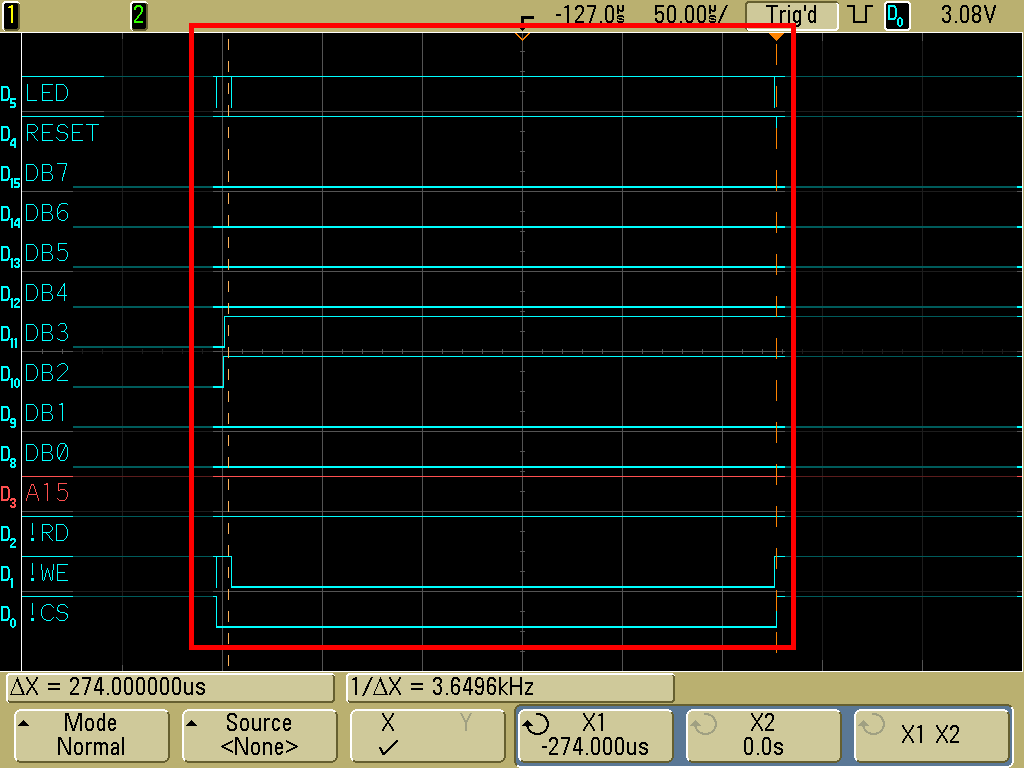
\includegraphics[width=1\textwidth]{TeilA/print_34_dip.png}}
	\caption{SSD1963 mit GPIO}
			\label{fig:ssd1963_gpio}
		\end{subfigure}


        \begin{subfigure}[htp]{1\textwidth}
%\begin{figure}[h!]
	\centering
\fbox{	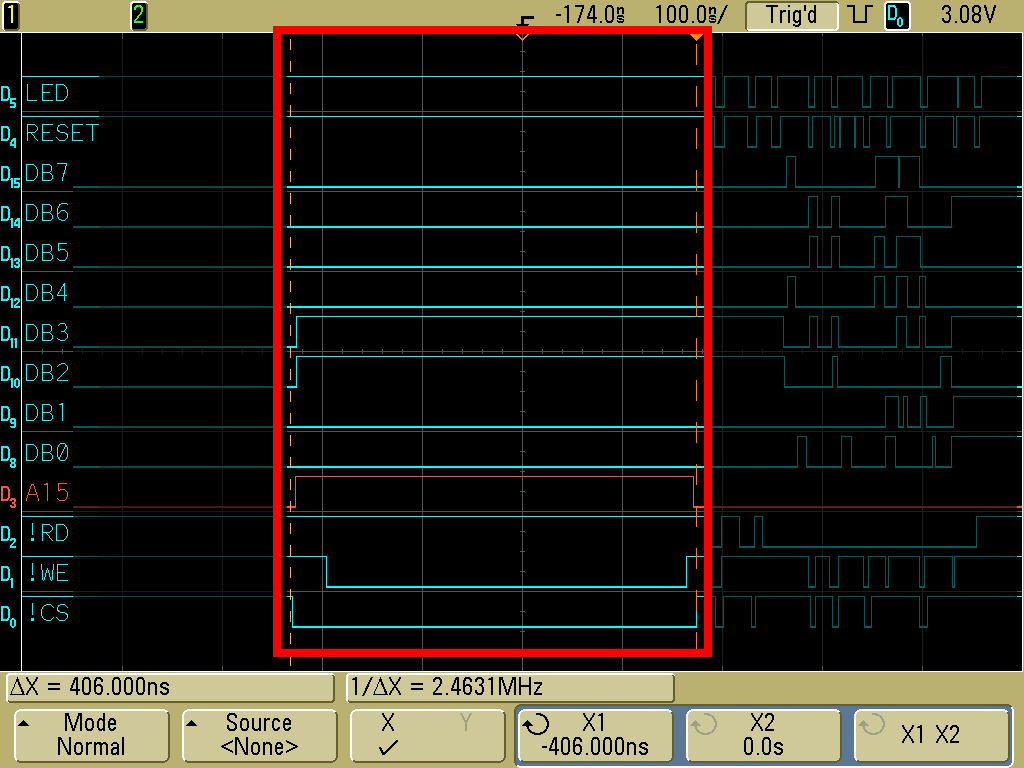
\includegraphics[width=1\textwidth]{TeilA/print_34_ext.png}}
	\caption{SSD1963 mit SRAM-Interface}
	\label{fig:ssd1963_sram}
\end{subfigure}

		\end{center}
\caption{SSD1963: Vergleich GPIO- und SRAM-Ansteuerung}
	\label{fig:ssd1963_gpio_sram}
\end{figure}
\newpage
Das geforderte Timing ist in \refa{fig:ssd1963_timing_constraints} zu sehen und beinhaltet die minimal notwendigen Zeiten zwischen den einzelnen Signalen.
\begin{figure}[htp]
%\begin{minipage}[t]{0.8\textwidth}
%\begin{figure}[h]
	\centering
\fbox{	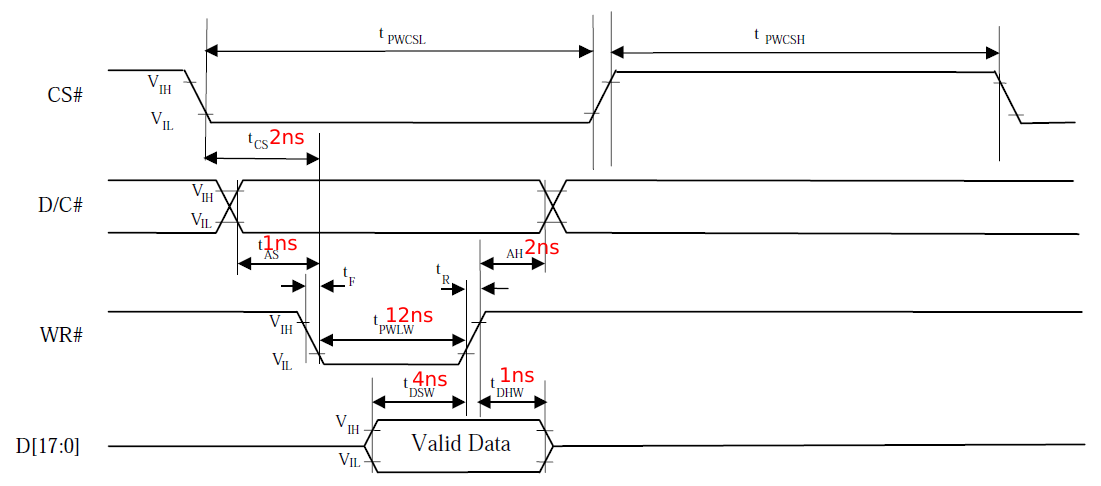
\includegraphics[width=1.0\textwidth]{TeilA/ssd1963_writeCycleConstraings.png}}
	\caption{8080-Timingbedingung für SSD1963}
	\label{fig:ssd1963_timing_constraints}
\end{figure}
Diese Mindestzeiten wurden innerhalb der Oszilloskopbilder eingehalten und verifiziert, sodass ein Fehler mit dem Protokoll des 8080-Interface ausgeschlossen werden kann. Bezüglich der uninitialisierten PLL des Displays und der verringerten Schreibrate ist in \refa{fig:ssd1963_sram} eine Chip-Select-Laenge von 406~Nanosekunden erkennbar, was einer Schreibgeschwindigkeit von 2.46~MHz entspricht. Dies ist weit unter den geforderten 5~MHz im uninitialisierten Zustand. Ein zu schnelles Schreiben ist in diesem Fall ebenfalls ausgeschlossen. Nachdem verifiziert wurde, dass aus der Adapterplatine vom Gnublin Extended die richtigen Signale geliefert werden, bleibt als Ursache nur noch das Display selbst. Da die Leitungsführung des ursprünglich verwendeten 4.3"' Displays nicht optimal ist, bei dem die 8080-Leitungen quer über die Platine geführt und im Anschluss von den RGB-Signalen im 90 Grad Winkel gekreuzt werden, wurde der Fehler im schlechten Platinendesign des Displays gesucht. Aufgrund dessen fand das 5"' Display mit demselben Controller Verwendung, das eine optimierte Leitungsführung besitzt. Jedoch waren die aufgeführten Lösungsansätze nicht zielführend, weswegen das Display nicht mit dem Gnublin Extended unter Verwendung des SRAM-Interface einsetzbar ist.

\input{Inhalt/TeilA/TeilAZusammenfassung}

